\section{Research Methodology}
\label{sec:Res}
\par  Portfolio construction depends heavily on how risk is defined and measured. Although mean-variance optimisation remains a classical benchmark, variance treats upside and downside deviations symmetrically and may therefore understate the practical importance of severe losses during turbulent market conditions [1], [3]. By contrast, Conditional Value-at-Risk (CVaR) focuses on the average loss beyond the VaR threshold and has been widely adopted in portfolio research as a downside-risk measure that is more sensitive to tail losses [1]–[3]. However, much of the recent literature applies CVaR within complex optimisation settings such as copula-based models, evolutionary algorithms, robust optimisation, or deep reinforcement learning [2]–[6]. This makes it less clear whether a simpler and more transparent CVaR-minimisation framework can already provide meaningful downside-risk benefits when compared with standard benchmark strategies.

\par In view of this problem, the present study examined whether portfolio construction based on CVaR-minimisation offers stronger downside-risk protection than Equal-Weight and Minimum-Variance strategies in a Malta-accessible UCITS ETF basket. The comparison is conducted under identical long-only and fully invested conditions using secondary historical ETF data and rolling out-of-sample backtesting. This design allows the effect of the portfolio-construction rule to be examined more directly, while keeping the dataset, constraints, and testing framework consistent across all strategies [5], [6].

\par The main hypothesis of this study states that, when applied to the same Malta-accessible UCITS ETF basket under identical rolling out-of-sample backtesting conditions, a CVaR-minimised portfolio will achieve lower CVaR and lower maximum drawdown than Equal-Weight and Minimum-Variance portfolios, without material deterioration in CAGR or Sharpe ratio. The corresponding null hypothesis states that no meaningful difference will exist among the three strategies in terms of CVaR, maximum drawdown, or risk-adjusted performance. This hypothesis is testable through empirical investigation because the independent variable is the portfolio-construction rule, while the dependent variables are the observed portfolio outcomes measured through predefined financial metrics [1], [5].

\par In light of the above, the aim of this research is to assess whether a simpler and more transparent CVaR-minimisation framework can provide stronger downside-risk protection than Equal-Weight and Minimum-Variance portfolio construction in a Malta-accessible UCITS ETF basket. More specifically, the study seeks to implement the three strategies under identical long-only and fully invested conditions and to evaluate their out-of-sample performance over the 2016–2025 period. The expected outcome is a clear empirical comparison showing whether CVaR-minimisation improves downside-risk measures such as CVaR and maximum drawdown, while preserving broadly competitive return and risk-adjusted performance. 
\par The research objectives were as follows:
\begin{enumerate}
    \item Construct a consistent historical dataset for the selected Malta-accessible UCITS ETF basket and prepare it for portfolio backtesting. 
    \item Implement Equal-Weight, Minimum-Variance, and CVaR-minimisation portfolio-construction rules under identical investment constraints. 
    \item Conduct rolling out-of-sample backtesting to evaluate how the three strategies perform across different market conditions over 2016–2025.
    \item Compare the strategies using return, volatility, risk-adjusted, and downside-risk measures, namely CAGR, volatility, Sharpe ratio, Sortino ratio, VaR, CVaR, and maximum drawdown.
    \item Assess whether CVaR-minimisation provides materially stronger downside-risk control than the benchmark strategies without significant deterioration in return-based performance.
\end{enumerate}

\par The research questions addressed in this study are organised around the data, portfolio-construction process, and evaluation stages identified in Section II. Since the present research does not propose a new complex optimisation engine, the questions are designed to examine whether a transparent benchmark comparison based on secondary ETF data can produce meaningful evidence on downside-risk control. 
\par The research questions are as follows:
\begin{enumerate}
    \item Historical dataset: What historical ETF dataset and investable UCITS ETF basket are most suitable for a controlled comparison of Equal-Weight, Minimum-Variance, and CVaR-minimisation strategies in a Malta-accessible setting? 
    \item process / candidate techniques: Under identical long-only and fully invested constraints, how does CVaR-minimisation compare with Equal-Weight and Minimum-Variance as a portfolio-construction approach? 
    \item evaluation and testing: How does the proposed CVaR-minimisation strategy compare with the benchmark strategies in rolling out-of-sample backtesting when evaluated using CAGR, volatility, Sharpe ratio, Sortino ratio, VaR, CVaR, and maximum drawdown? 
\end{enumerate}

\subsection{Research Pipeline}

\par To answer the above research questions, the study was structured around the research pipeline illustrated in Fig. 3. The first stage consisted of defining the six-ETF UCITS basket and collecting the historical adjusted closing prices required for the backtest. The second stage involved aligning prices across common trading dates, checking completeness, handling missing observations, and deriving periodic returns from the cleaned series. The third stage consisted of constructing Equal-Weight, Minimum-Variance, and CVaR-minimisation portfolios under identical long-only and fully invested constraints. The fourth stage involved rolling out-of-sample backtesting, where portfolio weights were estimated from the preceding in-sample window and then applied to the subsequent out-of-sample period until the end of 2025. The final stage consisted of evaluating realised portfolio outcomes using CAGR, annualised volatility, Sharpe ratio, Sortino ratio, VaR, CVaR, and maximum drawdown, and comparing the CVaR strategy against the benchmark portfolios.

\begin{figure}[H]
  \centering
  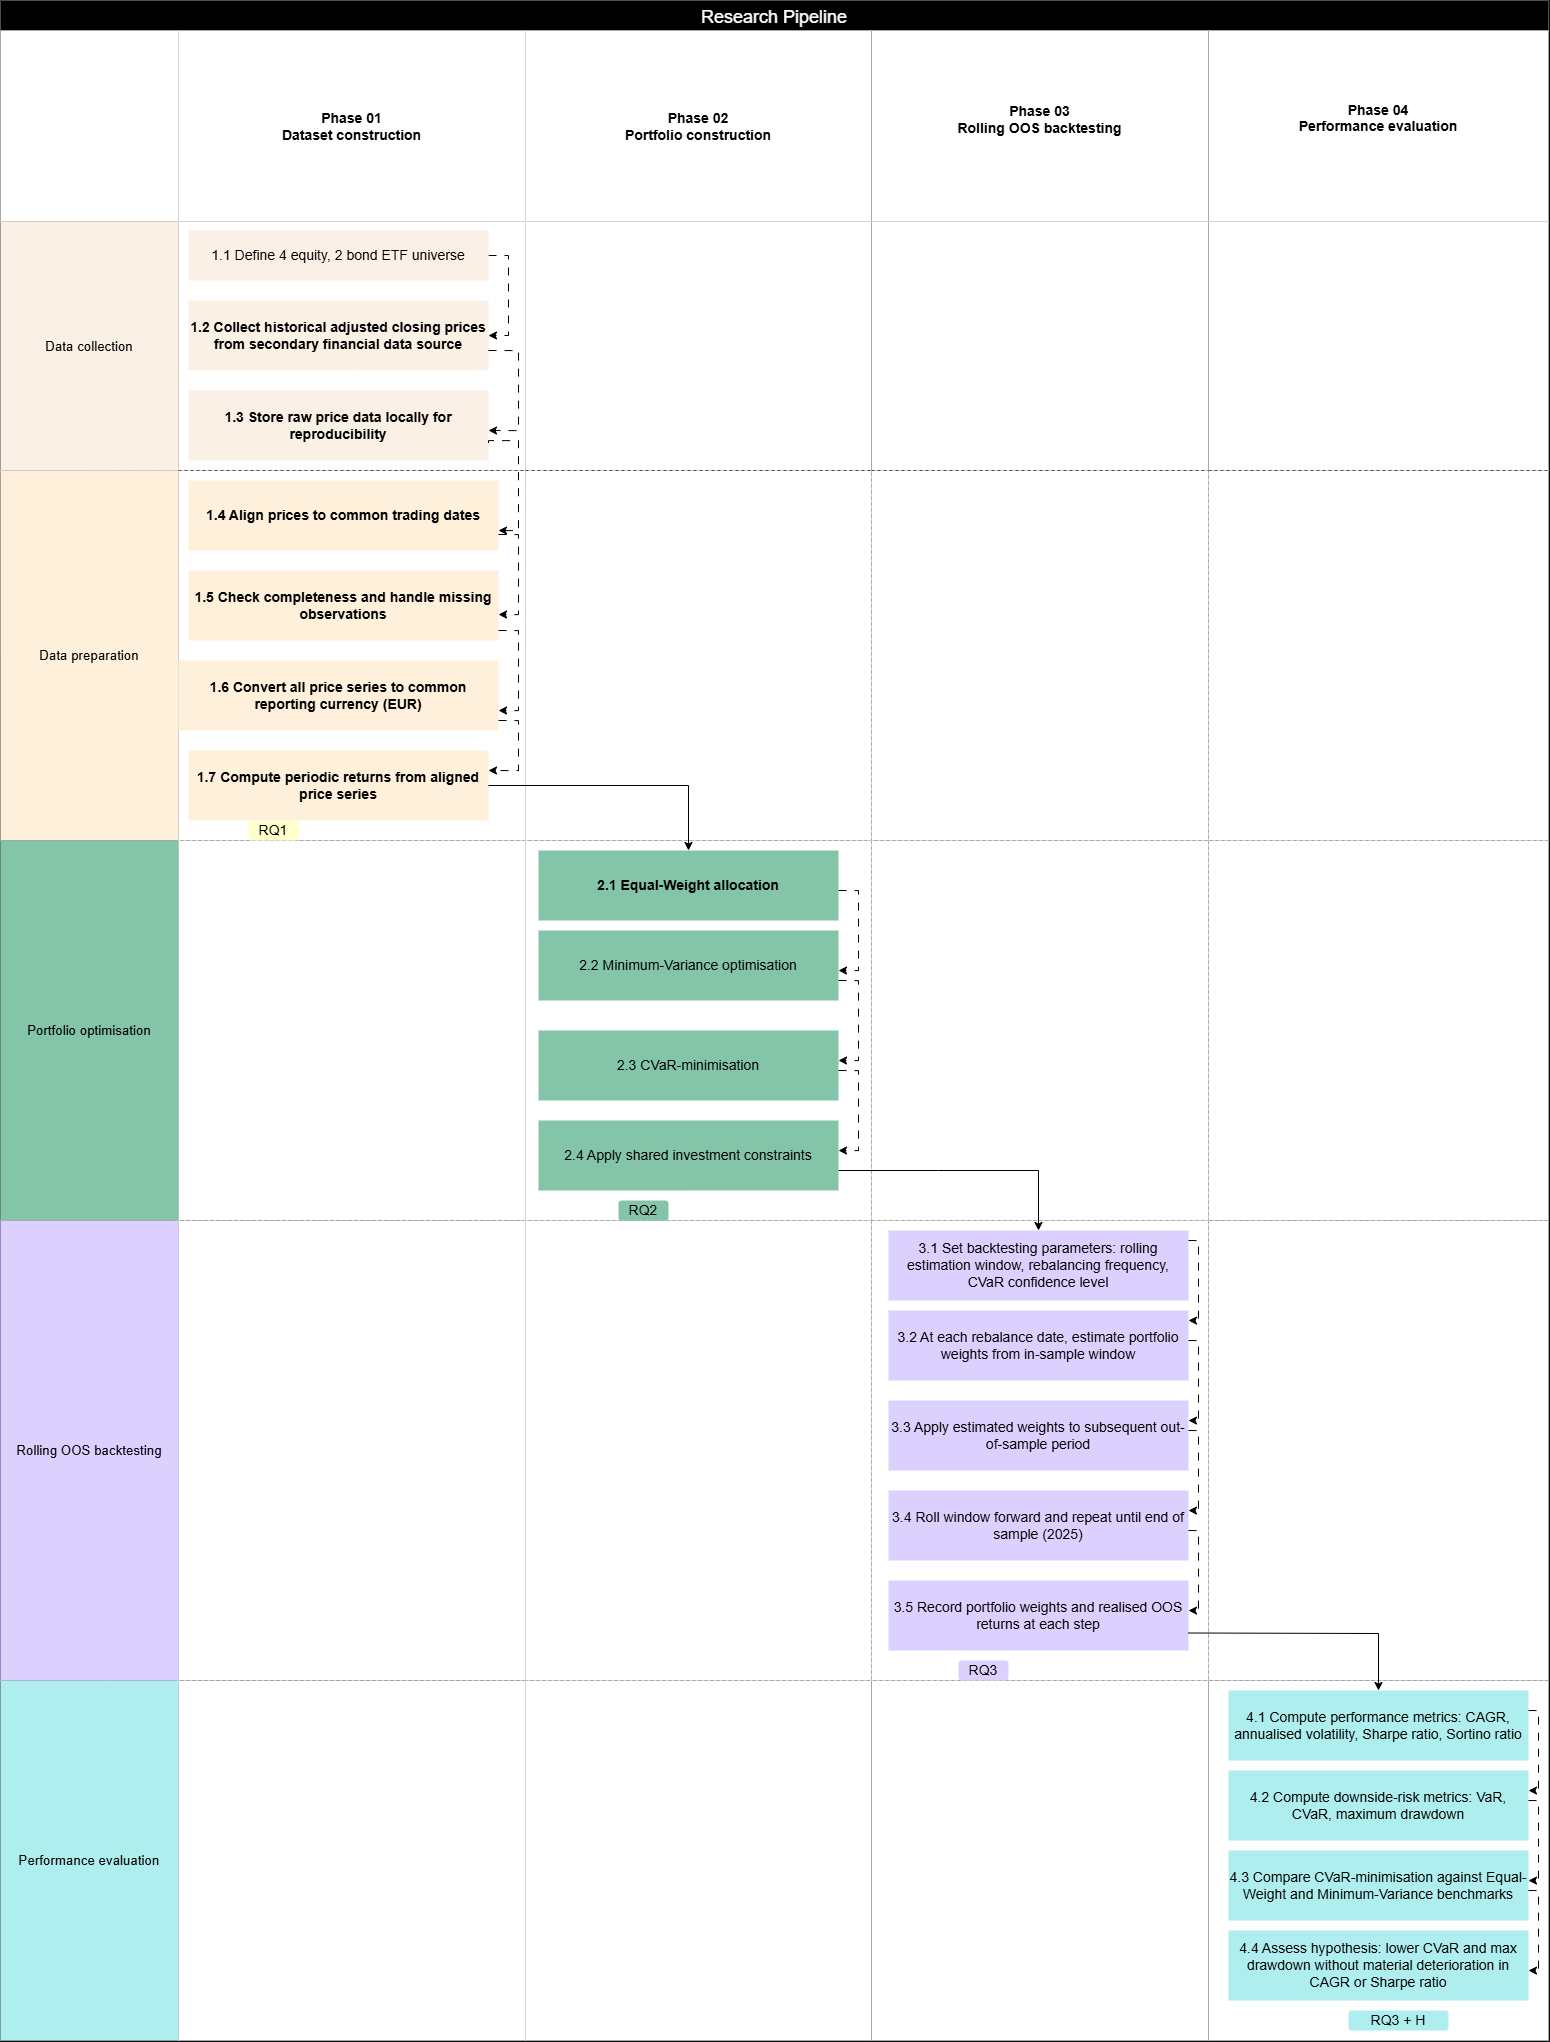
\includegraphics[width=\columnwidth]{includes/pipeline4.png}
  \caption{Fig. 3. Research pipeline for CVaR-based portfolio optimisation in a Malta-accessible UCITS ETF basket.}
  \label{fig:pipeline}
\end{figure}
\FloatBarrier

\subsection{Research Approach and Experimental Variables}
\begin{table}[!t]
    \centering
    \caption{Experimental variables in the present study}
    \label{tab:ExpVars}
    \footnotesize
    \setlength{\tabcolsep}{4pt}
    \renewcommand{\arraystretch}{1.15}
    \begin{tabular}{p{0.28\columnwidth}|p{0.28\columnwidth}|p{0.38\columnwidth}}
    \textbf{Variable type} & \textbf{Variable} & \textbf{Operationalisation} \\ \hline
    Independent variable & Portfolio-construction strategy & Equal-Weight, Minimum-Variance, CVaR-minimisation. \\ \hline
    Dependent variables & Portfolio outcomes & CAGR, annualised volatility, Sharpe ratio, Sortino ratio, VaR, CVaR, maximum drawdown. \\ \hline
    Control variables & ETF universe & Fixed six-ETF Malta-accessible UCITS basket. \\ \hline
    Control variables & Data treatment & Adjusted closing prices, common trading dates, identical return-construction procedure. \\ \hline
    Control variables & Investment constraints & Long-only, fully invested. \\ \hline
    Control variables & Backtesting settings & Same rolling estimation logic, rebalancing structure, and evaluation period for all strategies. \\
    \end{tabular}
\end{table}
\FloatBarrier

\par The present study adopted a positivist philosophy, a deductive approach, and a mono-method quantitative design. This choice was appropriate because the research aimed to test whether changing the portfolio-construction rule produced measurable differences in objectively observed portfolio outcomes. More specifically, the study employed a controlled experimental backtesting strategy using secondary historical ETF data. This design was methodologically suitable because the ETF universe, data treatment, and investment constraints were held constant, while the portfolio-construction rule was varied across Equal-Weight, Minimum-Variance, and CVaR-minimisation. In this way, the study was designed to isolate the effect of the optimisation approach as clearly as possible.
\par The independent variable in the study was the portfolio-construction strategy, operationalised through three portfolio rules: Equal-Weight, Minimum-Variance, and CVaR-minimisation. The dependent variables were the observed portfolio outcomes, namely CAGR, annualised volatility, Sharpe ratio, Sortino ratio, VaR, CVaR, and maximum drawdown. To preserve comparability, the ETF universe, adjusted-price treatment, common-date alignment, long-only fully invested constraints, and the same rolling out-of-sample testing framework were treated as control variables. Since the study evaluated repeated portfolio outcomes over time rather than collecting subjective human responses, the design was consistent with a quantitative backtesting methodology.

\subsection{Dataset and Data Preparation}
\par The dataset used in this study consisted of secondary historical ETF market-price data for a fixed basket of six Malta-accessible UCITS ETFs, representing four equity sleeves and two government-bond sleeves. The selected basket comprised iShares Core S\&P 500 UCITS ETF USD (Acc), iShares Core MSCI Europe UCITS ETF EUR (Acc), iShares Core MSCI Japan IMI UCITS ETF, iShares Core MSCI Emerging Markets IMI UCITS ETF (Acc), iShares USD Treasury Bond 7–10yr UCITS ETF (Acc), and iShares Euro Government Bond 7–10yr UCITS ETF (Acc). ISINs were treated as the master identifiers for the basket, while EUR was used as the reporting currency for analysis.
\par Historical adjusted closing prices were downloaded as an exchange market-price dataset through the yfinance interface and stored locally for reproducibility. Adjusted prices were used because they provided a more consistent basis for return calculation than unadjusted closing prices. The raw data were then aligned across common trading dates, checked for completeness, and cleaned to handle missing observations before periodic returns were computed from the aligned series. This preparation stage was necessary to ensure that all three portfolio-construction rules were tested on the same underlying data under identical conditions.

\subsection{Portfolio-Construction and Rolling Out-of-Sample Backtesting}

\par Three portfolio-construction strategies were implemented in the study. Equal-Weight served as a transparent benchmark in which capital was allocated equally across all ETFs. Minimum-Variance represented the classical variance-based optimisation approach, while CVaR-minimisation represented the downside-risk approach under investigation. All three strategies were implemented under shared investment constraints so that no short selling was permitted and the full portfolio weight remained invested at each rebalance point. This ensured that the comparison remained controlled, interpretable, and directly aligned with the hypothesis.
\par To evaluate these strategies, the study employed rolling out-of-sample backtesting over the 2016–2025 period. At each rebalance date, portfolio weights were estimated from the preceding in-sample window and then applied to the subsequent out-of-sample holding period. The window was then rolled forward and the procedure repeated until the end of the sample. This design was preferred to a single in-sample optimisation because it reduced look-ahead bias and enabled repeated testing across different market conditions. In methodological terms, this rolling structure was also consistent with the evaluation patterns identified in the reviewed portfolio-optimisation literature.
\par A separate pilot study was not required because the research did not involve human participants, questionnaires, or competing candidate systems that first needed to be screened before main testing. Instead, preliminary implementation checks were carried out to verify price alignment, return calculation, optimisation constraints, and output consistency before running the full backtest. This was sufficient for establishing a stable quantitative workflow without introducing an unnecessary additional experimental phase.

\subsection{Performance Evaluation}

\par The realised out-of-sample portfolio results were evaluated using both return-oriented and downside-risk metrics. Return and risk-adjusted performance were assessed using CAGR, annualised volatility, Sharpe ratio, and Sortino ratio. Downside-risk behaviour was assessed using VaR, CVaR, and maximum drawdown. These measures were selected because the hypothesis did not claim that CVaR-minimisation would maximise return; rather, it tested whether downside-risk control could be improved without materially worsening return-based performance.
\par The analysis was primarily comparative. The EW, MV, and CVaR portfolios were compared under the same dataset, constraints, and backtesting logic, and the resulting metrics were interpreted relative to the hypothesis and to the benchmark-comparison designs discussed in Section II. This approach was consistent with the assignment guidance that findings should later be discussed honestly and compared with existing research rather than being presented as a perfect or universal solution.

\subsection{Validity, Reliability, Generalisability, Limitations, and Ethical Considerations}

\par The validity of the study was strengthened by the controlled design. All three portfolio rules were tested on the same ETF basket, over the same time horizon, using the same adjusted-price treatment, date alignment, and investment constraints. The main intentional source of variation was therefore the portfolio-construction rule itself. Reliability was supported through the use of fixed procedures for data preparation, return calculation, portfolio construction, and backtesting, together with local storage of the downloaded data for reproducibility. However, the generalisability of the findings remained bounded by the specific six-ETF UCITS basket, the 2016–2025 period, and the long-only fully invested framework used in the study.
\par The study also had several limitations. First, it relied on a relatively small and intentionally transparent ETF universe rather than a large institutional asset set. Second, portfolio outcomes depended on historical market behaviour and therefore could not guarantee future performance. Third, the backtest was based on market-price data and did not attempt to model every real-world friction in depth, such as taxes or all trading frictions. These limitations do not invalidate the study, but they do define the scope within which its conclusions should be interpreted.
\par Finally, the study raised minimal ethical risk because it used secondary historical financial data and did not involve human participants, interviews, surveys, or personal data. The main ethical obligations were therefore academic honesty, correct citation, transparent reporting of the method, and accurate acknowledgment of the data source and implementation choices. This is consistent with the wider MCAST guidance that methodology should be rigorous, clearly explained, and properly referenced.
